% Setup - do not change
\documentclass[11pt]{article}
\usepackage[top=0.9in, left=0.9in, bottom=0.9in, right=0.9in]{geometry} 
\usepackage{parskip}

\usepackage[english]{babel}
\usepackage[utf8]{inputenc}
\usepackage{amsmath,amsthm,amssymb,graphicx,pdfpages,lipsum,hyperref}
\usepackage[none]{hyphenat}
\usepackage{csquotes}

\setlength\parindent{0pt}
%%%%%%%%%%%%%%%%%%%%%%%%%%%%%%%%%%%%%%%%%%%%%%%%%%%%%%%%%%%%%%%%%%%
% add other packages here if required

%% Bibliography are specified in this file. You can also choose inline bib style if you want to. But make sure your citation style is consistent (and proper)
% For more details on citation: https://library.unimelb.edu.au/recite
\usepackage[sorting = none]{biblatex}
\addbibresource{references.bib}

%%%%%%%%%%%%%%%%%%%%%%%%%%%%%%%%%%%%%%%%%%%%%%%%%%%%%%%%%%%%%%%%%%% the '%' symbol denotes comments

% Begin document creation
% DELETE THE \lipsum PLACEHOLDERS WHEN YOU BEGIN
\title{\textbf{Forecasting Rideshare service demand in NYC using statistical models under pandemic conditions} \\}
\author{
James Barro \\
Student ID: 1082092 \\
%% Replace the link with your github repo
% 1. Remember to escape underscore in the link.
% 2. Remember to include the commit you want to submit in the link
\href{https://github.com/MAST30034-Applied-Data-Science/mast30034-project-1-JamesB112}{Github Repository Link}
}

\begin{document}
\maketitle

\section{Introduction}
% Link to a 30 min tutorial if you require revision: https://www.overleaf.com/learn/latex/Learn_LaTeX_in_30_minutes

New York City (NYC) has gradually returned to a new \textit{normal} as the Covid-19 pandemic continues, but with the threat of new variants, and potential wide-spreading of other infectious diseases such as polio \cite{infectious}, a return to pre-pandemic conditions is not likely to occur any time soon. 

As some people still hold fear of catching the Covid-19 virus in confined spaces, Ridesharing services such as Uber and Lyft have suffered a slow recovery to pre-pandemic customer numbers, whilst registered drivers have dropped to the extent that a partnerships with NYC Yellow taxi have been made to fill shortages \cite{uber_article}. Additionally, with petrol prices still well above normal, and the nature of Rideshare services requiring individual drivers to maintain their own vehicles, it has become important for these companies to support their \textit{employees} as much as possible.

This report will assume the perspective of Rideshare service companies, with the intent to forecast the demand of customer demand by outlined pick-up locations around New York City (NYC). This is designed for mutual beneficiary, of registered drivers who can be strategically allocated to specific locations of future high demand, potentially reducing idle time (time between customer trips), whilst in-turn, boosting profits due to potentially more customer trip requests being served.

After prepossessing, joining and aggregating datasets described in section 2, Poisson and Negative Binomial regression models were fitted on 9 predictors over 40896 total records, with evaluated also conducted. These types of models were chosen in particular due to estimating each predictors (E.g. Time of day) affect on the target (Rideshare Service demand), which can give deeper insight other methods can not achieve (E.g. Neural Networks) (see section 4 Modeling for more details).

\section{Datasets}
The NYC Taxi \& Limousine Commission (NYCTLC) \cite{tlc} collects and publishes trip record information for each taxi and for-hire vehicle trip completed by licensed drivers and vehicles in NYC.

From this database, the High Volume For-Hire Vehicle (HVFHV) trip records, which includes records from popular Rideshare services such as Uber, has been utilised for this research project. Although many attributes for each trip have been captured, many were discarded due to  the nature of 'counting' trips to achieve aggregation statistics. To add dimensionality, external datasets deemed to have some relationship with Ridesharing service usage, and are outlined below.

\begin{enumerate} 
    \item Climate Dataset \cite{climate}: Contains various climate statistics recorded at an hourly rate from the JFK Airport weather station. Weather is perceived to not have a strong effect on service usage (as confirmed in ), but has been included due to containing several attribute that can be used to increase the dataset dimensional. 
    \item Covid-19 Dataset \cite{covid}: Contains Covid-19 case numbers from the beginning of the pandemic in the United States. As there is a strong likelihood that Covid-19 cases decrease demand, and the fact the investigation aims to create a model accounting for a changing pandemic situation, it is essential to include these statistics.
    \item Holiday data \cite{workalendar}: Contains dates of past and future public holiday dates for countries across the world. It also contains locally/nationally recognised public holidays in the state of New York, which have been extracted. This is used more for accounting for outliers (Days that happen to be public holidays), as service users may display different behaviours for these days.
\end{enumerate}

\subsection{Timeline Choice}
As Covid-19 pandemic conditions are factored into the modeling due to reasons outlined above, Rideshare service records from February 2020 (the month of the first case of Covid-19 in the United States of America) on-wards should be taken. To minimise the effects of early pandemic situations, and recognise the attitudinal shift of New York citizens following widespread distribution of certified vaccines, the most recent records available should be taken. To ensure the models takes into account recent trends, and ignores \textit{old} records, a rolling 6 month dataset was used, in particular, records from September 2021 to the end of February 2022. After fitting the models, records from March 2022 were used to test each models predictive power.

\subsection{Preliminary Analysis}
Figure 1 was plotted by counting all Rideshare service records by PULocationID (See documentation for further information \cite{tlc}), and provides a better understanding of hot-spots, low demand areas, and clustered regions in New York City. Firstly, indicated with markers, it can be observed that LaGuardia (top) and JFK airport's average rideshare demand is significantly higher than of most other locations in New York City (a cases to consider).  Another interesting observation to make, is that most PULocationID's neighbours share similar demand, creating a (hard to see) visual cluster (Take Staten island for example).

Considering the nature of Ridesharing apps, where users are able to draw registered drivers to their respective location, and the visual \textit{clustering} of nearby PULocationIDs, the Zone clustering attribute 'Borough\_Zone' (see section 3.2) was created to cluster taxi demand by the Boroughs of New York City. In other words, the assumption that registered drivers can be allocated to each defined area (in Borough\_Zone), where then they are then spread  uniformly over the geological area like a \textbf{net}, has been made. This due to the following considerations:
\begin{itemize}
    \item The demand may vary by PULocationID over time, hence to better reduce variance in our predictions, like locations should be grouped
    \item To account for cases where registered drivers patrolling one PULocationID receive a ride request from a neighbouring Location
\end{itemize}

Please note, under these assumptions above, rideshare records from Newark Airport (PULocationID 1) were removed, due to lying independent (isolated) from other Zones, hence the assumption of a \textbf{net} cannot hold.

\begin{figure}[h]
    \centering
    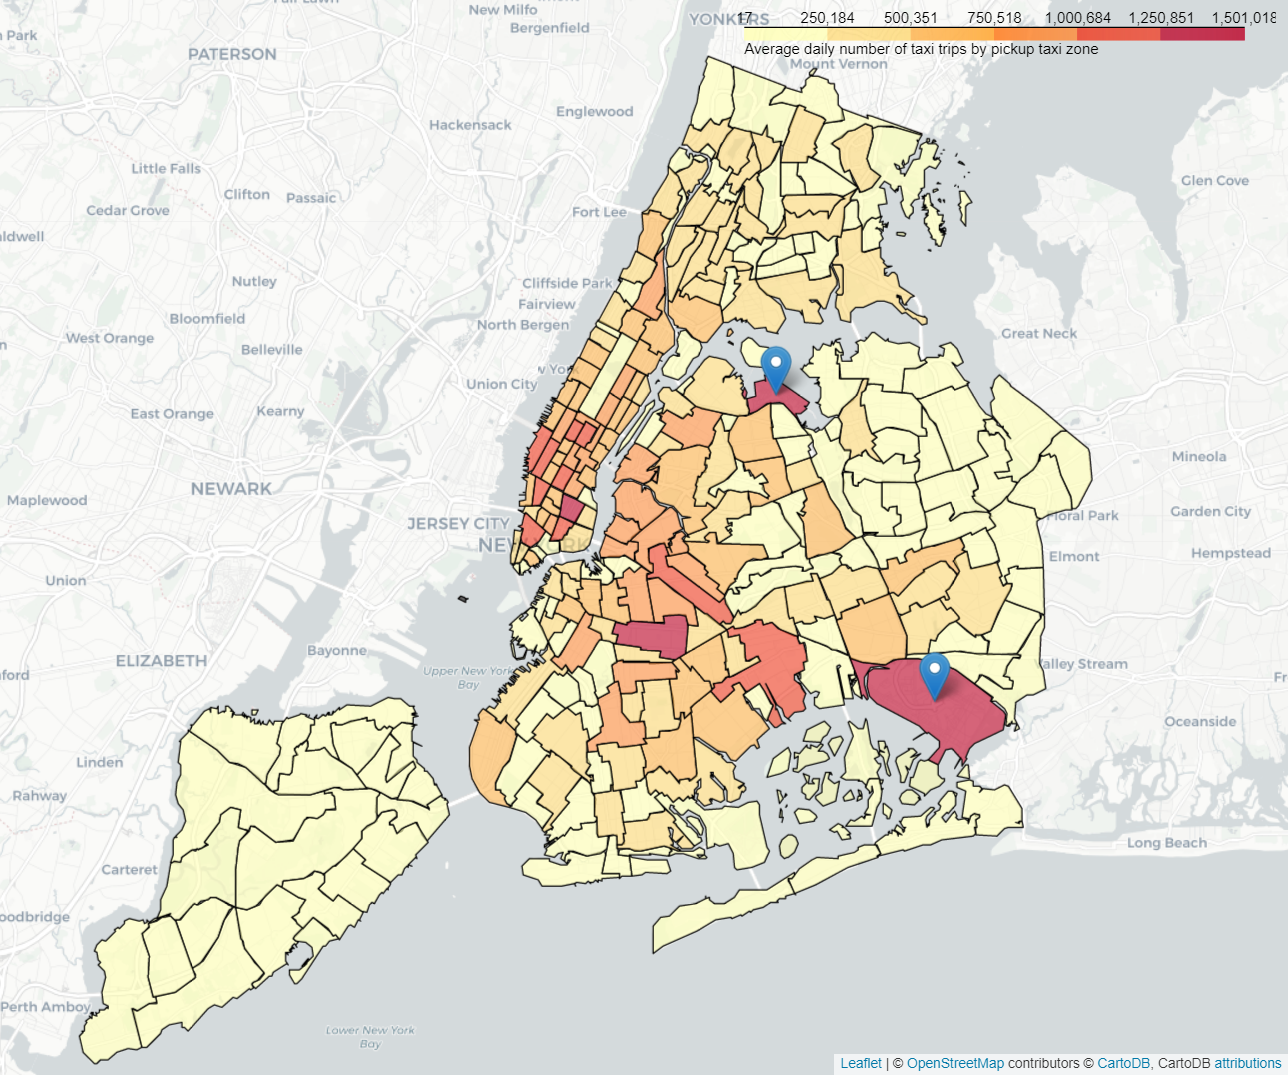
\includegraphics[width=12cm]{plots/Average_Taxi_Demand_Per_Day.PNG}
    \caption{Average Daily Total Pickups by Rideshare PULocationID Between 09-2021, 02-2022 (inc.) } % refer to this image as (Figure 1)
\end{figure}

\section{Preprocessing}
\subsection{Rideshare Data}
Rideshare records from the HVFHV dataset were loaded and filtered under the following conditions below. The motivation behind these filtering methods were to ensure that recorded trips were removed due to tangible attributes being out of distribution (for further information on attributes, refer to \cite{tlc}.
\begin{itemize}
    \item \textbf{trip\_times}: over 3 hours and less than 1 minute trips were removed. The upper limit is due to the fact that it takes around 2 hours to drive from one side of New York to the other (in a straight line), then to account for traffic, 3 hours is achieved. The lower limit is to account for very short or canceled trips, which should not be counted. This is because the driver is only unavailable to take surrounding requests for a very small time. 
    \item \textbf{trip\_distance}: needs to be positive. This is to account for cases where the meter was left on, or potentially incorrectly recorded trip records (negative values)
    \item \textbf{trip\_cost} is not \$0 USD. As there may be loopholes in the app to cause trips to be ‘free’. This do not fit the goal of fitting a model, which can forecast \textbf{profitable} trips
    \item \textbf{PULocationID} and \textbf{DOLocationID} are described in the integer range 2-263 for locations accros NYC (exclusion of ID 1 explained previously) Trips that drop off out of this range are removed to suit the described \textbf{net}.
\end{itemize}

Additionally, attributes from eternal datasets from earlier were loaded and reformatted into formats compatible with our models:


Climate Dataset
\begin{itemize}
    \item \textbf{TMP}: The atmospheric temperate, at a given time 
    \item \textbf{WND}: The strength of the wind, at a given time
    \item \textbf{DEW}: The dew point, at a given time
\end{itemize}
Holiday Dataset
\begin{itemize}
    \item \textbf{Holiday}: A Boolean attribute, indicating if a given day is a public holiday
\end{itemize}
Covid-19 Dataset
\begin{itemize}
    \item \textbf{Covid-19\_7AVG}: The rolling 7 day average of Covid-19 cases in New York City
\end{itemize}

\subsection{Feature Engineering}
The following features were created for the purpose of preforming aggregation on specific attributes, as well as for the final modeling.
\begin{itemize}
    \item \textbf{Borough\_Zone}: This was created by taking all possible combinations of the \textit{Borough} and \\
    \textit{Service\_Zone} attribute from the taxi-lookup file \cite{tlc}. JFK and LaGuardia Airport also had there own separate zones, as they were identified as outliers in section 2.2
    \item \textbf{Hour}: This was extracted from the Pickup\_datetime attribute in HVFHV. It was later converted to categorical data, as from figure 2, it can be observed that service demand does vary across the day, hence more useful at a catergorical variable than a continuous one
    \item \textbf{Day}: This is a categorical variable for the day of the week (E.g Monday). As it can be said peoples schedules change from day to day, it is would be beneficial to capture this information. 
    \item \textbf{Date\_seq}: As \testit{time series} data is being modeled, a variable capturing the order of each record being recorded should be included. It is of type int, and signifies the number of days since September 1st 2021
    \item \textbf{Count}: This represents the demand of valid rideshare service trips, the target of our models, which is a aggregated statistics from derived on the grouping on Date, Hour and Borough-Zone.
\end{itemize}
From figure 2, it can be observed that the the categories 'Manhattan\_Yellow Zone' and 'Manhattan\_Boro Zone' do have concerningly large confident interval widths, and suggests the PULocationID zones under the category have high variance. On the other hand, Staten Island looks to fit service demand nicely, whilst the treatment of the 2 airports as separate labels appears useful, as they are shown to have vastly different demand distribution over the day shown. However, considering other predictors, such as Day, Covid-19\_7AVG, have not been accounted for, let us perform modeling for a clearer understanding.
\begin{figure}[h]
    \centering
    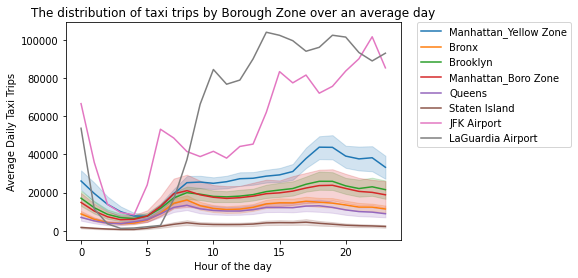
\includegraphics[width=12cm]{plots/Borough_Zone_Distribution.png}
    \caption{The Viability of grouping PULocationID zones into larger defined regions of Borough\_Zone categories. The Hue around each Borough\_Zone line plot is a 95 percent confidence interval for capturing respective Rideshare PULocationID recordings)}
 % refer to this image as (Figure 1)
\end{figure}

Please note, feature selection was performed in the Modeling section

\section{Modelling}
\subsection{Poisson Regression}
The Poisson regression model was modeled with the following formula, which uses a log link function.
\begin{align*}
    \tag{Model 1}
        log(Count) \sim Intercept + Date\_seq + Day + Borough\_Zone + DEW + \\TMP                 + WND + holiday + Covid-19\_7AVG + Hour
\end{align*}

The Poisson model is derived from the following source \cite{model_pois}. Even though this model is design for count target scenarios, which through aggregation has been achieved for our modeling dataset (the demand of ride services), the model assumption of independent observations on the other hand is broken (see figure 2's dependence on Hour of day), but this does not prevent the model from being used. 

\subsection{Interaction} 
Before model analysis, interaction between attributes was first investigated to produce the best possible version of the model to be analysed. The interaction terms Day:Borough\_Zone, holiday:Borough\_Zone, Hour:Day,  Covid-19\_7AVG:Day, 
Hour:Borough\_Zone, Hour:TMP, Hour:WND and Hour:DEW were all included due to realistically potential interaction between the sets of predictors. For example, the Day:Borough\_Zone term was chosen, as the day of the week may affect each Borough-Zone differently, which can improve estimating the target Count (rideshare services demand).

\begin{table}[h]
\centering
\begin{tabular}{||c c c c c||} 
 \hline
  & Resid. Df & Resid. Dev & Df Deviance  & Deviance\\ [0.5ex] 
 \hline\hline
  & 34901 & 7496415.8 &  &  \\ 
 \hline
 Interaction & 34478 & 2259988.23 & 423 & 5236427.57 \\
 \hline
\end{tabular}
\caption{\label{tab:table-name}Anova table reflecting the significance of including interactive terms in Model 1}
\end{table}

From Table 1, it can be observed that the interaction terms reduces Model 1's Residual Deviance by approximately 65 \%, which suggests that the terms are significant and should be included in the Final model. 
\begin{multline*}
    \tag{Model 1 Interaction}
        log(Count) \sim Intercept + Date\_seq + Day + Borough-Zone + DEW + TMP + WND + \\holiday + Covid-19\_7AVG + Hour + Day:Borough\_Zone + holiday:Borough\_Zone +\\ Hour:Day +  Covid-19\_7AVG:Day +
        Hour:Borough\_Zone + \\Hour:TMP + 
        Hour:WND + Hour:DEW
\end{multline*}


Upon reflecting on the unusually high Residual Deviance, it was thought the high count target attribute values could be the cause, as borough-Zone does take into account large areas of New York City. But upon reviewing the design of Poisson regression the assumption $E[\mathbf{Count}] &= Var[\mathbf{Count}]$ may not hold. Calculating these values for our dataset gives respective values 2328.54 and 7244890, which does indicate that the assumption is violated. However, a quasipoisson regression model can be used to estimate a dispersion parameter, which takes into account the violation of the assumption.
\subsection{Negative Binomial Regression}
To ensure that the Poisson regression model (with dispersion estimation) was still adequate, a negative binomial regression model \textit{count} was also fitted for comparison. This model does not suffer the broken Poisson model assumption described. The formula for this model was taken as the same as Model 1 Interaction, as like Poisson, they can both utilise \textit{log} link function, whilst the interaction terms have already been deemed significant. This will be defined as Model 2

\subsection{Model Comparison & Evaluation}
After fitting each model, including refitting Model 1 Interaction to estimate the dispersion parameter, which will be referred to as \textbf{Model 1 Final}, both models indicated good fits, but with Model 2 appearing more suitable from figure 3. 
\begin{figure}[h]
\centering

\caption{Comparision of model diagnosis plots for Model 1 Final (left) vs Model 2 (Right) }
 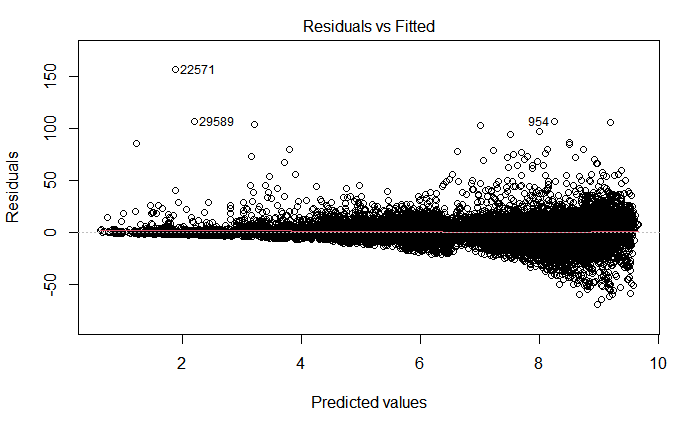
\includegraphics[width=65mm]{plots/Pois_plot_1.png}
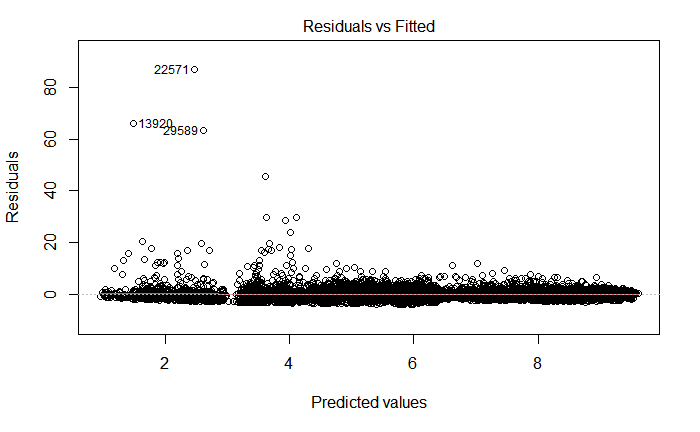
\includegraphics[width=65mm]{plots/Neg_Bin_plot_1.png}
\hspace{0mm}

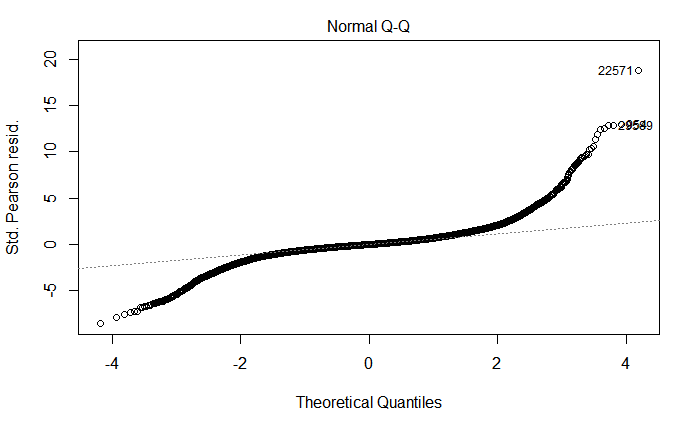
\includegraphics[width=65mm]{plots/Pois_plot_2.png}
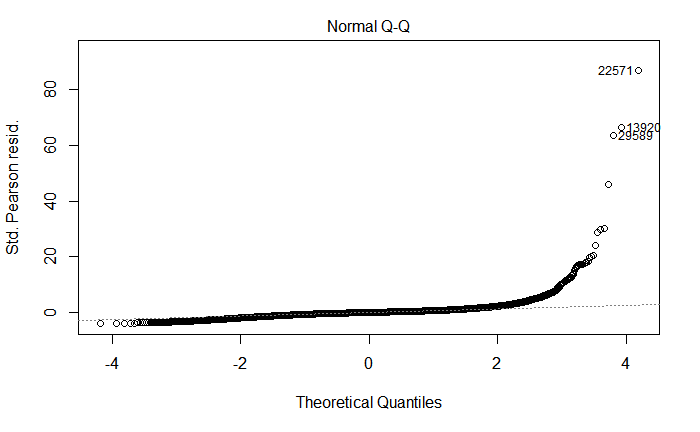
\includegraphics[width=65mm]{plots/Neg_Bin_plot_2.png}
\end{figure}
\subsubsection{Residual vs Fitted}
Examining this plot for both models, Model 2 residuals are more closely pack around zero, whilst Model 1 Interaction is more loose. However, both models overall have a very small average Residual Difference , as observed by the line of best fit (red) remaining close to zero, which suggests they both provide a good fit. 
\subsubsection{Q-Q Plot}
The Q-Q plots are much more revealing than the previous plot type. Comparing the two models, Model 2's ordered Quantile match the standard residuals nicely, except for the strong tail, which suggests the model tends to under estimate. On the other hand, Model 1 has weak tails at either end of the Q-Q plot, which suggests it is does not suffer from general over or under estimation, but as accurate as Model 1 interaction.
\subsection{Prediction Evaluation}
To understand the predictive power of both models, the prediction of a future rideshare service demand was analysis. As the models were trained on data from September 2021 to end of February 2022, the Hourly demand was estimated for March 1st 2022 for Brooklyn (then next day. Brooklyn was taken arbitrarily).

Figure 4 shows that Model 2 under estimate almost all the hourly recordings. On the other Hand, Model 1 follows the distribution quite accurately between the hours 5-9 and 13-18, but lack accuracy outside these intervals. 
\begin{figure}[h]
    \centering
    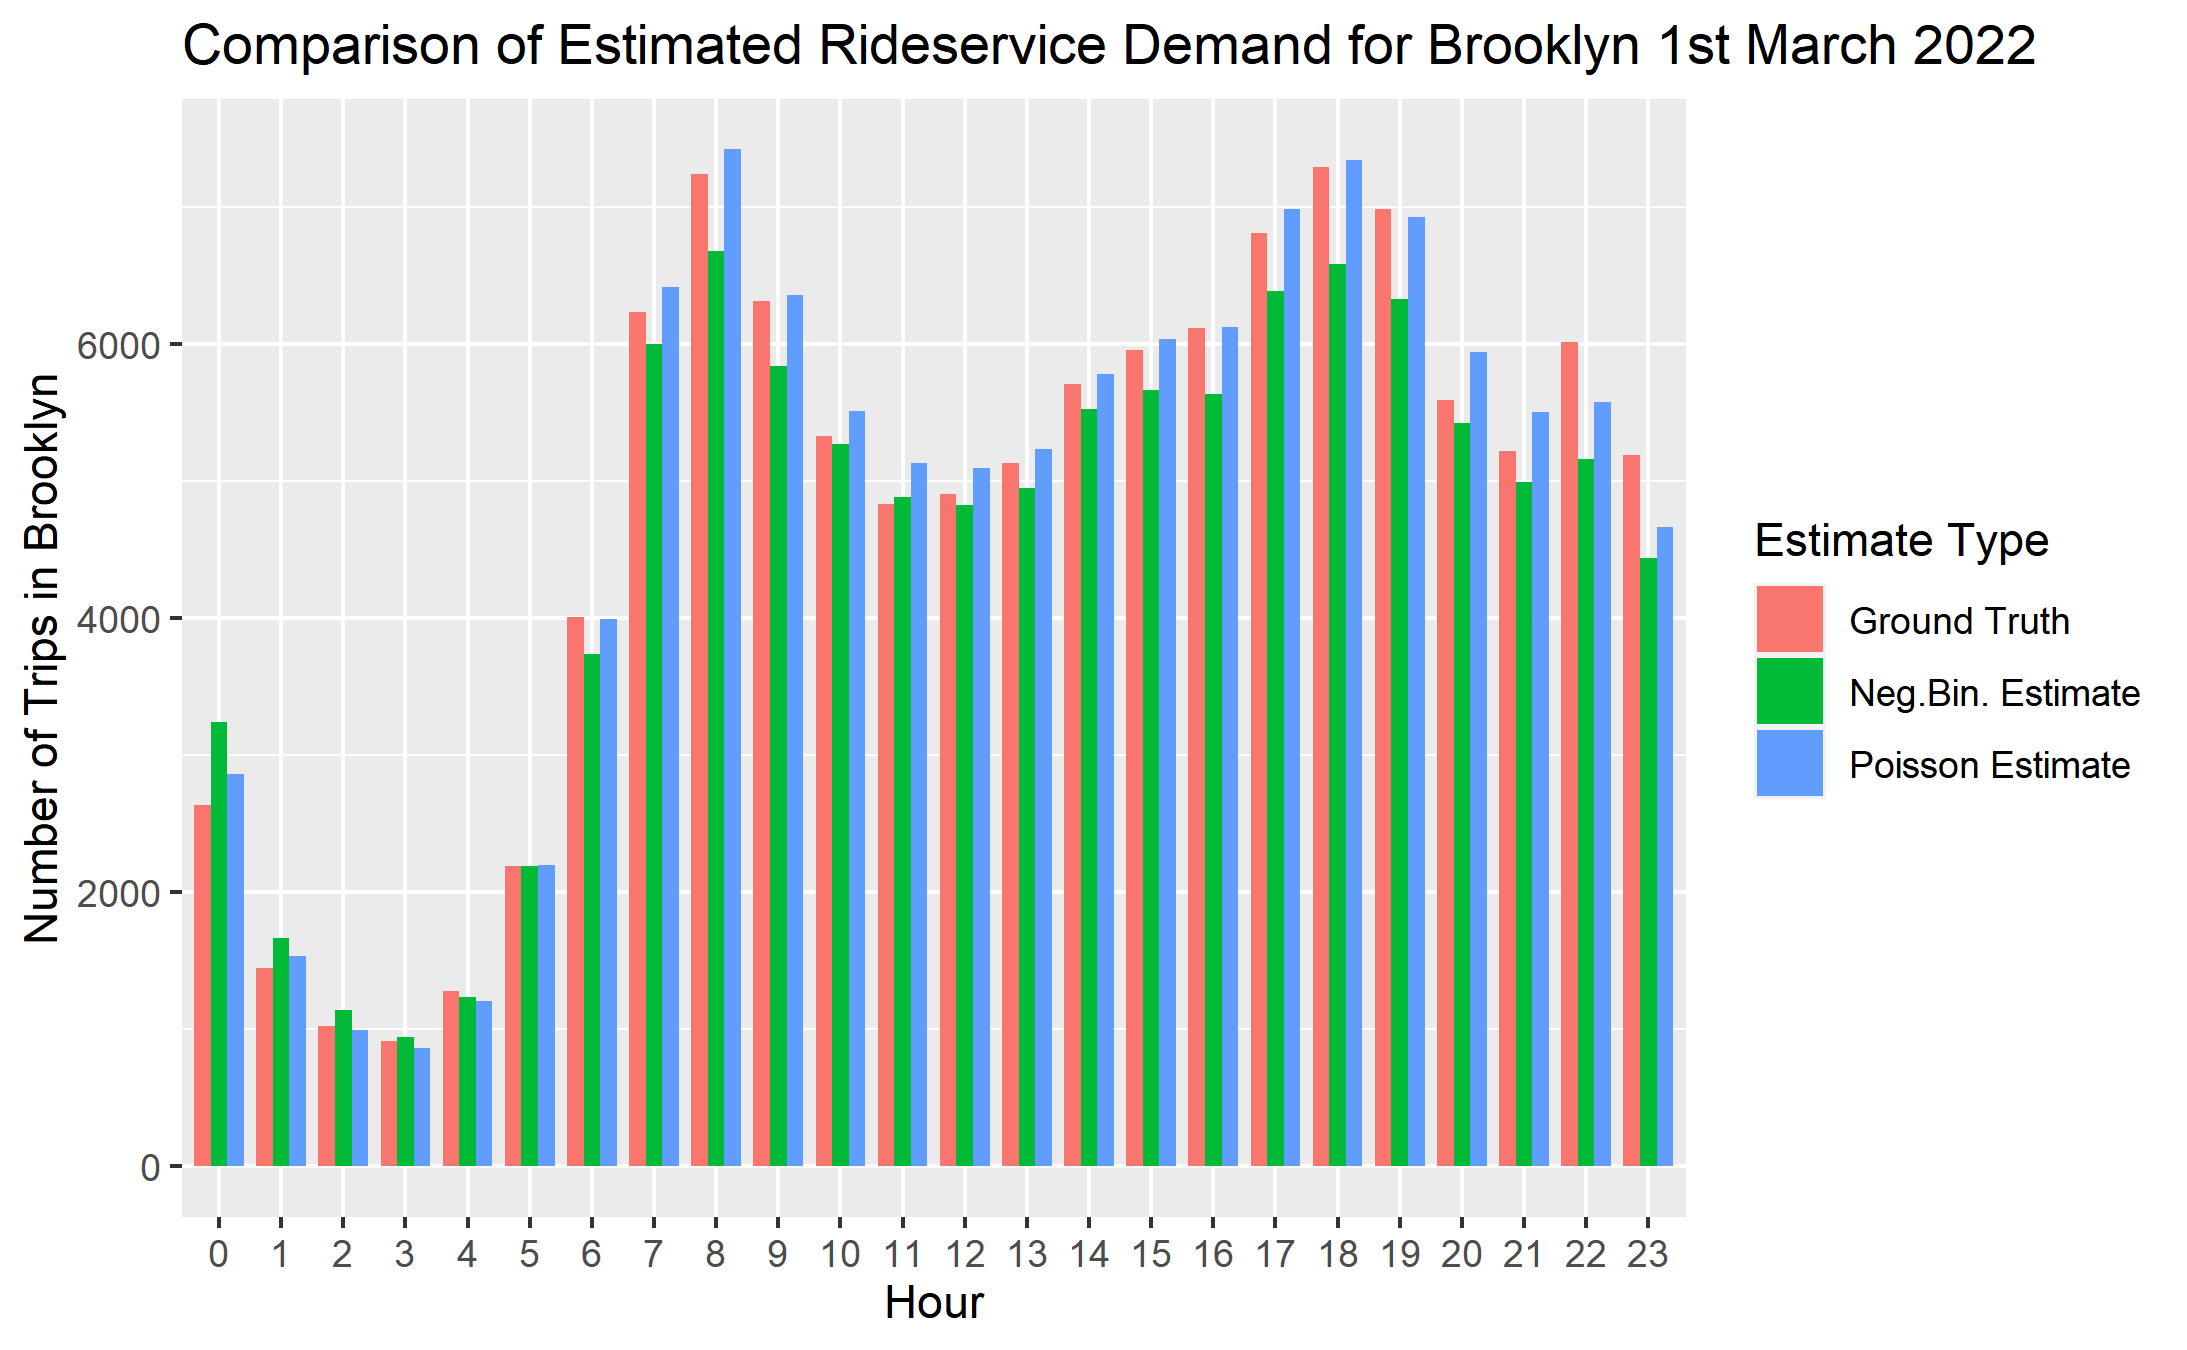
\includegraphics[width=12cm]{plots/March_1st_2022_Brooklyn_Prediction.png}
    \caption{Displays the difference between Model 1 \& 2's predicted Hourly demand estimates with the True value for March 1st 2022}
 % refer to this image as (Figure 1)
\end{figure}

Despite the promising accuracy of Model 1 in figure 4, Model 2 may be preferred due to the diagnosis plots indicating a better fitting model on the training dataset. Although, further prediction analysis would be required to get a proper indication of which model is preferred. 

\subsection{Feature analysis}
Table 2 indicates that all the predictor attributes in the aggregated modeling dataset are significant. Although DEW and WND have the weakest significance, there p vales remain below the 0.1 significance level, and furthermore their presence as interaction terms suggest they should remain in the model. As expected, the Covid\_19 estimate suggests that cases do reduce the demand for rideshare services, whilst TMP is also strongly significant, with the estimate suggesting warmer weather is better. However, it can likely be said that the some of the estimates in table 2 will change drastically if the dataset was taken over the period March 2022 - August 2022, due to seasonal different. In other words, as the model selected is over the winter season, it would be interesting to see the change for warmer seasons. 
\begin{table}[h]
\centering
\begin{tabular}{||c c c c c||} 
 \hline
 Predictor & Estimate &  Std. Error & t value & Pr(\|t\|)\\ [0.5ex] 
 \hline\hline
 (Intercept) & 7.346e+00 & 2.397e-02 & 306.436 & 0.000e+00  \\ 
 \hline
 Date\_seq & 8.427e-04 & 3.548e-05 & 23.750 & 1.083e-123 \\
 \hline
 DEW  & -2.075e-03 & 1.151e-03 & -1.802 & 7.154e-02 \\
 \hline
 TMP & 7.954e-03 &  1.400e-03 & 5.680 & 1.360e-08 \\
 \hline
 WND & 2.656e-03 & 1.633e-03 &  1.627 & 1.038e-01 \\
 \hline
 holidayTrue  & 3.135e-02 & 1.023e-02 & 3.065 & 2.176e-03 \\
 \hline
 Covid\_7AVG & -4.941e-06 & 2.031e-07 & -24.331 & 1.138e-129 \\
 \hline
\end{tabular}
\caption{\label{tab:table-name}Model 1 Interaction estimates of predictor variables with respective significance tests (excl. Hour and Borough\_Zone)}
\end{table}


\section{Discussion}
The fact that a Poisson Regression model is able to predict demand for specified Borough\_Zones in NYC with a low average error per hour, is impressive. Although, an improved investigation into this model type should be taken, including the viability of aggregating Count by \textit{PULocationID}. The inclusion of extra features, such as School-Holiday, Number of public events per PULocationID would also provide further insight of service demand  distributions for rideshare companies. Furthermore, deeper outlier should have been taken, as filtering was made without examining attribute distributions.

With the improvement in mind and the report's positive findings, it should be suggested that rideshare companies should attempt to implement their own demand predicting models. This is because this data can then be fed to individual registered drivers for better geological spacing across New York City. This would provide better opportunities for drivers to earn money faster (reduce the time and fuel spent between rides delivered), in turn increasing profits for the rideshare company. 

% BEGIN REFERENCES SECTION
\printbibliography

\end{document}

